\documentclass[10pt,a4paper]{article}

\usepackage[a4paper,margin=22mm,headheight=14pt]{geometry}
\usepackage[T1]{fontenc}
\usepackage{lmodern}
\renewcommand{\familydefault}{\sfdefault}
\usepackage{amsmath,amssymb}
\usepackage{booktabs}
\usepackage{longtable}
\usepackage{graphicx}
\usepackage{microtype}
\usepackage{xcolor}
\usepackage{caption}
\usepackage[numbers,sort&compress]{natbib}
\usepackage{fancyhdr}
\usepackage[hidelinks]{hyperref}

\definecolor{navy}{HTML}{214B6B}
\hypersetup{colorlinks=true,linkcolor=navy,citecolor=navy,urlcolor=navy}
\captionsetup{font=small,labelfont={bf,color=navy},justification=justified,hypcap=false}
\graphicspath{{figures/}}
\pagestyle{fancy}
\fancyhf{}
\fancyhead[L]{\small SafeEdit-CRE supplementary information}
\fancyhead[R]{\small Computational regulatory-sequence design}
\fancyfoot[C]{\thepage}

\title{\textbf{Supplementary Information}\\[0.35em]
\large SafeEdit-CRE: uncertainty-aware cross-model selection improves minimal regulatory-DNA editing for cell-type-specific design}
\author{Angran Xia\\
School of Chemistry and Chemical Engineering, Shaanxi Normal University,\\
620 West Chang'an Avenue, Chang'an District, Xi'an, Shaanxi 710119, China\\[0.35em]
\textit{Correspondence:} \texttt{haangyeon@snnu.edu.cn}}
\date{}

\begin{document}
\maketitle
\tableofcontents
\clearpage

\section{Supplementary methods and audit notes}

\subsection{Study phases and separation of roles}

The study was executed in sequential phases. G0--G3 established the data audit,
published-model reproduction, pilot CNN reviewer, and initial editing workflow. G4
froze a 96-parent, three-method hard-audit benchmark. G6 assigned computational
candidate tiers. G7 trained the full-data residual-dilated reviewer and the
multi-kernel post-freeze evaluator. G8 selected 600 new parents and compared four search
methods. G9 reran seven complete search configurations on 180 parents. G10 applied
the post-freeze endpoint and assembled summary analyses. Activity labels were never used
to select parents or candidate sequences.

The terms \emph{reviewer} and \emph{post-freeze evaluator} denote different roles. The
reviewer was available to SafeEdit during G8/G9 search. The post-freeze evaluator was
loaded only after candidate files were frozen. Both were trained on the same public
MPRA source table; hence ``post-freeze'' describes procedural separation from search, not
external biological independence.

\subsection{Integrity checks}

The final G9 table contains 15,120 rows, 180 unique parents, seven configurations,
three target cells, and four budgets. There are no duplicate
parent--target--budget--configuration keys, no non-finite numeric values, and no exact
edit-budget violations among feasible designs. The G8 collapsed table contains
28,800 method-level rows and 600 parents. Random metrics are means of three independent
replicates; the collapsed table must not be used to select a particular DNA sequence.

All submission payloads were rechecked after manuscript generation. The release
manifest contains SHA-256 checksums for every payload file and excludes the manifest
itself from self-hashing.

\section{Supplementary results}

\subsection{Data partitions and predictor performance}

\begin{table}[ht]
\centering
\caption{Quality-filtered full-data partitions used for G7 model training.}
\label{tab:splits}
{\small
\begin{tabular}{lrrp{4.5cm}}
\toprule
Partition & Records & Chromosomes & Use \\
\midrule
Training & 627,661 & Eligible chromosomes excluding validation/test & Parameter fitting \\
Validation & 58,811 & 19, 21, X & Checkpoint choice and variance scaling \\
Test & 62,582 & 7, 13 & Final predictive diagnostics \\
\midrule
Total & 749,054 & -- & After quality filtering and exact deduplication \\
\bottomrule
\end{tabular}
}
\end{table}

\begin{table}[ht]
\centering
\caption{Ensemble performance on the 62,582-record test split, recomputed from saved
candidate-independent prediction tables.}
\label{tab:modelperf}
\begin{tabular}{llrrrr}
\toprule
Model & Cell & Pearson $r$ & Spearman $\rho$ & MAE & Uncertainty--error $\rho$ \\
\midrule
Reviewer & K562 & 0.845 & 0.781 & 0.396 & 0.448 \\
Reviewer & HepG2 & 0.855 & 0.809 & 0.354 & 0.404 \\
Reviewer & SK-N-SH & 0.847 & 0.810 & 0.390 & 0.399 \\
\addlinespace
Post-freeze evaluator & K562 & 0.785 & 0.719 & 0.463 & 0.467 \\
Post-freeze evaluator & HepG2 & 0.795 & 0.743 & 0.417 & 0.416 \\
Post-freeze evaluator & SK-N-SH & 0.799 & 0.760 & 0.444 & 0.400 \\
\bottomrule
\end{tabular}
\end{table}

\begin{table}[ht]
\centering
\caption{Validation-scaled interval coverage on the test split.}
\label{tab:coverage}
\begin{tabular}{llrrr}
\toprule
Model & Cell & 80\% interval & 90\% interval & 95\% interval \\
\midrule
Reviewer & K562 & 0.815 & 0.897 & 0.935 \\
Reviewer & HepG2 & 0.794 & 0.885 & 0.930 \\
Reviewer & SK-N-SH & 0.814 & 0.900 & 0.940 \\
\addlinespace
Post-freeze evaluator & K562 & 0.821 & 0.900 & 0.935 \\
Post-freeze evaluator & HepG2 & 0.789 & 0.879 & 0.923 \\
Post-freeze evaluator & SK-N-SH & 0.816 & 0.899 & 0.935 \\
\bottomrule
\end{tabular}
\end{table}

\begin{figure}[ht]
\centering
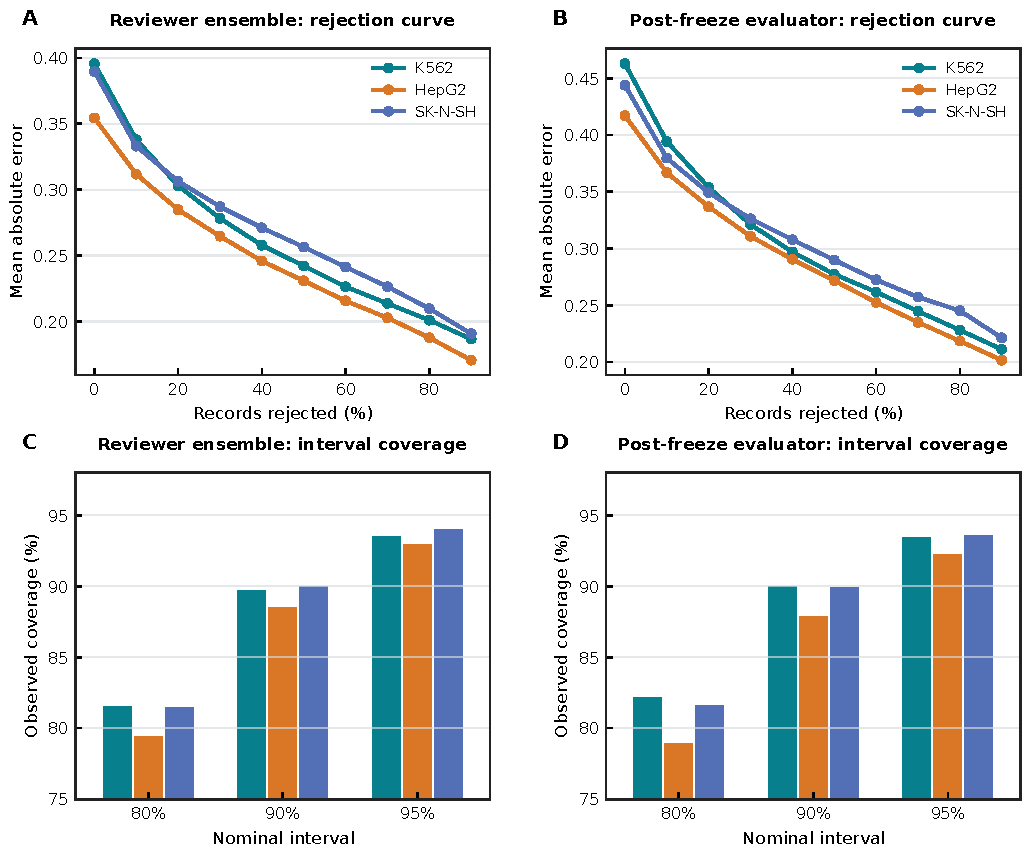
\includegraphics[width=\textwidth]{figS2_uncertainty_rejection.pdf}
\caption{\textbf{Uncertainty rejection and interval calibration.} \textbf{A--B}, mean
absolute error for the reviewer and post-freeze ensembles as records with the largest
predicted uncertainty are removed from the held-out test set. \textbf{C--D}, observed
test coverage at 80\%, 90\%, and 95\% nominal levels by cell type. Curves and bars are
descriptive test diagnostics; variance scales were fixed from validation only.}
\label{fig:s2}
\end{figure}

\clearpage
\subsection{G4 hard-audit stratification}

\begin{longtable}{llrrrr}
\caption{G4 audit pass rates by target cell and edit budget. Each row contains 96
paired parents per method.}\label{tab:g4strata}\\
\toprule
Target & Budget & Random (\%) & Greedy (\%) & SafeEdit (\%) & SafeEdit--Greedy (pp) \\
\midrule
\endfirsthead
\toprule
Target & Budget & Random (\%) & Greedy (\%) & SafeEdit (\%) & SafeEdit--Greedy (pp) \\
\midrule
\endhead
K562 & 1 & 14.6 & 59.4 & 60.4 & 1.0 \\
K562 & 5 & 8.3 & 57.3 & 78.1 & 20.8 \\
K562 & 10 & 17.7 & 41.7 & 83.3 & 41.7 \\
K562 & 20 & 25.0 & 50.0 & 82.3 & 32.3 \\
HepG2 & 1 & 10.4 & 34.4 & 35.4 & 1.0 \\
HepG2 & 5 & 5.2 & 37.5 & 47.9 & 10.4 \\
HepG2 & 10 & 2.1 & 31.3 & 58.3 & 27.1 \\
HepG2 & 20 & 8.3 & 28.1 & 59.4 & 31.3 \\
SK-N-SH & 1 & 25.0 & 35.4 & 39.6 & 4.2 \\
SK-N-SH & 5 & 16.7 & 35.4 & 57.3 & 21.9 \\
SK-N-SH & 10 & 14.6 & 21.9 & 66.7 & 44.8 \\
SK-N-SH & 20 & 8.3 & 30.2 & 68.8 & 38.5 \\
\bottomrule
\end{longtable}

\subsection{G8 post-freeze endpoint and heterogeneity}

\begin{table}[ht]
\centering
\caption{Pooled G8 method summaries. Each method has 7,200 parent--target--budget
records after averaging the three random replicates.}
\label{tab:g8summary}
\begin{tabular}{lrrrr}
\toprule
Method & Margin gain & Target gain & Positive margin (\%) & Uncertainty \\
\midrule
Random matched & 0.001 & 0.012 & 48.6 & 0.185 \\
Greedy Malinois & 0.822 & 1.803 & 97.1 & 0.329 \\
Primary beam & 0.881 & 1.866 & 94.8 & 0.335 \\
SafeEdit consensus & 0.877 & 1.661 & 95.4 & 0.314 \\
\bottomrule
\end{tabular}
\end{table}

\begin{table}[ht]
\centering
\caption{Pooled paired G8 contrasts. Differences are SafeEdit minus comparator;
confidence intervals use 100,000 parent-cluster bootstrap replicates.}
\label{tab:g8paired}
\begin{tabular}{llrr}
\toprule
Comparator & Metric & Mean difference & 95\% CI \\
\midrule
Greedy & Post-freeze margin gain & 0.0555 & 0.0398 to 0.0705 \\
Greedy & Post-freeze target gain & $-0.1412$ & $-0.1774$ to $-0.1057$ \\
Greedy & Post-freeze uncertainty & $-0.0153$ & $-0.0214$ to $-0.0091$ \\
\addlinespace
Primary beam & Post-freeze margin gain & $-0.0036$ & $-0.0114$ to 0.0042 \\
Primary beam & Post-freeze target gain & $-0.2048$ & $-0.2294$ to $-0.1808$ \\
Primary beam & Post-freeze uncertainty & $-0.0209$ & $-0.0251$ to $-0.0166$ \\
\addlinespace
Random matched & Post-freeze margin gain & 0.8763 & 0.8562 to 0.8960 \\
Random matched & Post-freeze target gain & 1.6494 & 1.6034 to 1.6950 \\
Random matched & Post-freeze uncertainty & 0.1285 & 0.1222 to 0.1348 \\
\bottomrule
\end{tabular}
\end{table}

\clearpage
\begin{center}
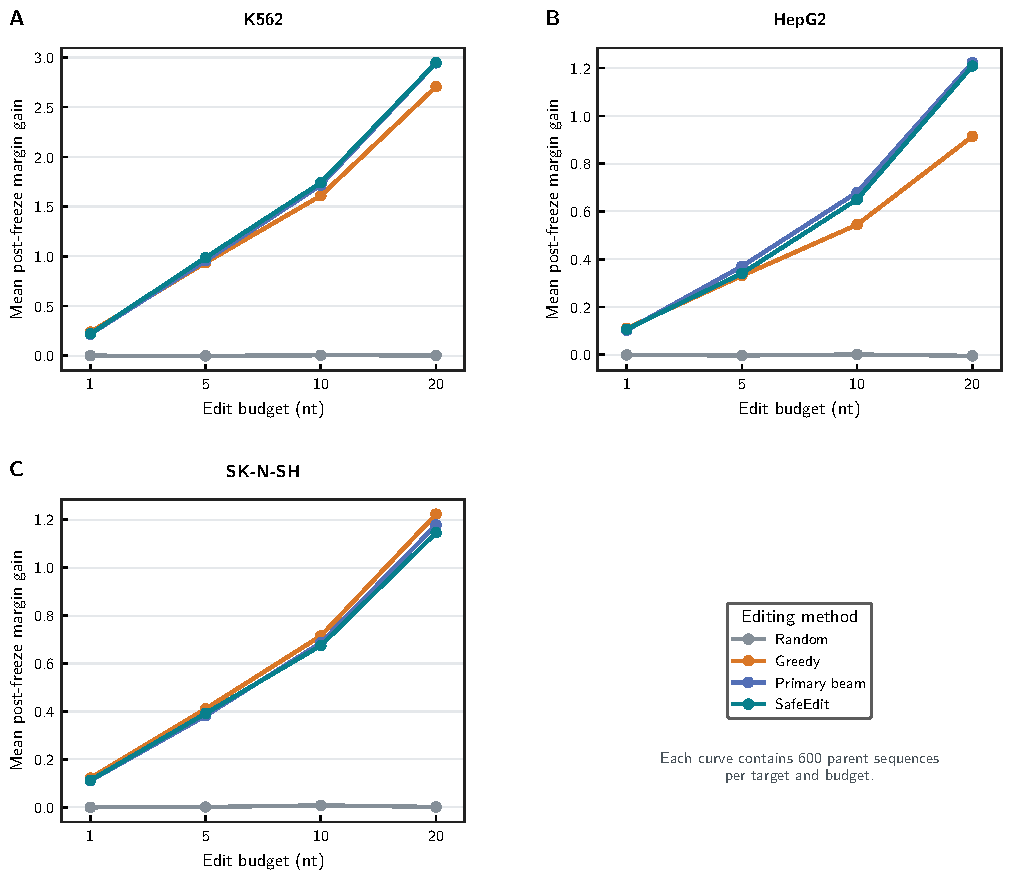
\includegraphics[width=0.96\textwidth]{figS4_stratified_effects.pdf}
\captionof{figure}{\textbf{Target--budget heterogeneity in the G8 post-freeze endpoint.}
\textbf{A--C}, mean post-freeze specificity-margin gain across edit budgets for random,
greedy, primary-beam, and SafeEdit searches in K562, HepG2, and SK-N-SH. Each point
summarizes 600 parents. Values are descriptive and are not multiplicity-adjusted.}
\label{fig:s4}
\end{center}

\clearpage
\subsection{G9 true-search ablation}

\begin{table}[ht]
\centering
\caption{G9 post-freeze outcomes for seven independently rerun search configurations.
Each configuration contains 2,160 rows from 180 parents, three targets, and four
budgets.}
\label{tab:g9summary}
\begin{tabular}{lrrrrr}
\toprule
Configuration & Margin gain & Target gain & Positive (\%) & Uncertainty & Infeasible \\
\midrule
Primary beam & 0.890 & 1.897 & 94.7 & 0.334 & 48 \\
SafeEdit full & 0.890 & 1.705 & 95.3 & 0.312 & 48 \\
No reviewer score & 0.890 & 1.897 & 94.7 & 0.334 & 48 \\
No uncertainty penalty & 0.891 & 1.719 & 95.2 & 0.313 & 48 \\
No strand penalty & 0.887 & 1.701 & 95.4 & 0.310 & 48 \\
No naturalness rerank & 0.979 & 2.017 & 95.3 & 0.343 & 48 \\
No sequence prefilter & 0.910 & 1.763 & 98.1 & 0.318 & 0 \\
\bottomrule
\end{tabular}
\end{table}

\begin{table}[ht]
\centering
\caption{Selected G9 paired contrasts. Differences are full SafeEdit minus the
ablation; intervals use 100,000 parent-cluster bootstrap replicates.}
\label{tab:g9paired}
\begin{tabular}{llrr}
\toprule
Comparator & Metric & Mean difference & 95\% CI \\
\midrule
Primary beam & Post-freeze margin gain & 0.0002 & $-0.0145$ to 0.0151 \\
Primary beam & Post-freeze target gain & $-0.1920$ & $-0.2440$ to $-0.1432$ \\
Primary beam & Post-freeze uncertainty & $-0.0212$ & $-0.0283$ to $-0.0140$ \\
\addlinespace
No naturalness & Post-freeze margin gain & $-0.0888$ & $-0.1022$ to $-0.0754$ \\
No naturalness & Post-freeze target gain & $-0.3117$ & $-0.3600$ to $-0.2658$ \\
No naturalness & Post-freeze uncertainty & $-0.0305$ & $-0.0394$ to $-0.0218$ \\
\addlinespace
No prefilter & Post-freeze margin gain & $-0.0198$ & $-0.0387$ to $-0.0043$ \\
No prefilter & Post-freeze target gain & $-0.0581$ & $-0.1021$ to $-0.0227$ \\
No prefilter & Post-freeze uncertainty & $-0.0060$ & $-0.0102$ to $-0.0024$ \\
\bottomrule
\end{tabular}
\end{table}

\subsection{Candidate library}

\clearpage
\begin{center}
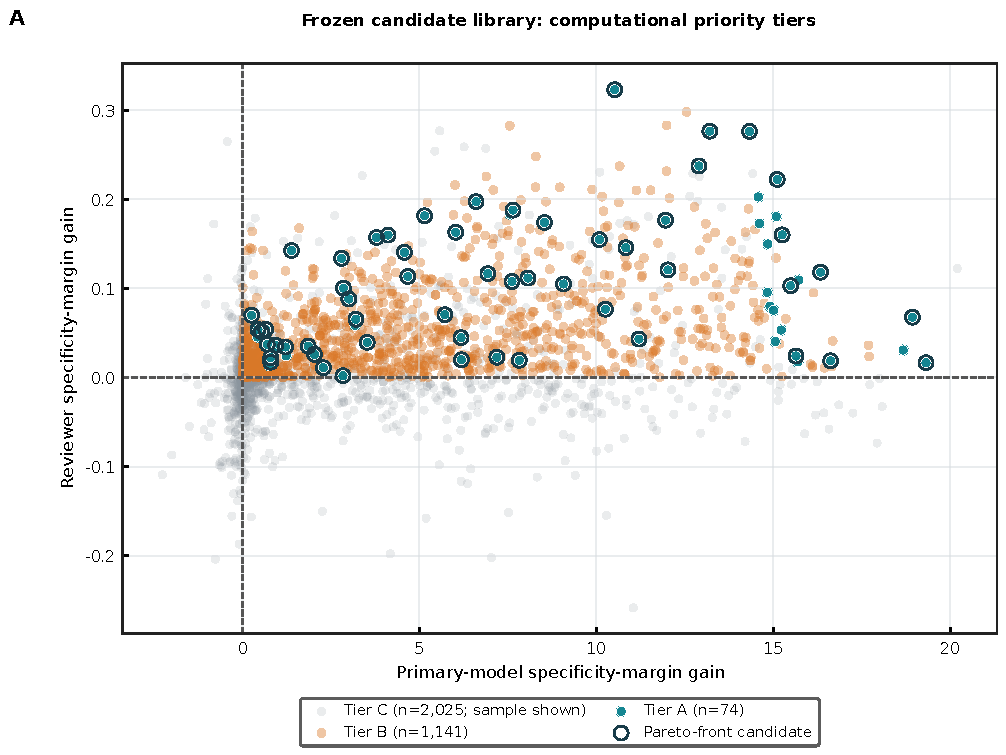
\includegraphics[width=0.86\textwidth]{figS3_candidate_tiers.pdf}
\captionof{figure}{\textbf{Computational candidate tiers.} Primary-model and reviewer
specificity-margin gains are shown for the frozen 3,456-sequence G4 library. All Tier
A and Tier B candidates are plotted; Tier C is downsampled for legibility. Outlined
points lie on the computed Pareto frontier. Tier labels represent computational
priorities for experimental screening.}
\label{fig:s3}
\end{center}

\begin{table}[ht]
\centering
\caption{Frozen G4 candidate tiers.}
\label{tab:tiers}
\begin{tabular}{lrrl}
\toprule
Tier & Candidates & Fraction (\%) & Intended use \\
\midrule
A & 78 & 2.3 & Highest-priority experimental panel \\
B & 1,224 & 35.4 & Alternative computational candidates \\
C & 2,154 & 62.3 & Method and failure-mode analysis \\
\bottomrule
\end{tabular}
\end{table}

\subsection{Representative Tier A candidates}

\begin{longtable}{p{1.8cm}p{1.8cm}p{1.8cm}p{1.8cm}p{1.8cm}p{1.8cm}p{1.8cm}}
\caption{Three representative Tier A experimentally actionable candidates, one per cell
type, selected from the locked non-overlapping 96-parent nine-criterion design benchmark.
Representative examples were selected according to a prespecified rule requiring Tier A
status, one example per target cell, positive cross-model margin gain, reduced
uncertainty, and no synthesis-risk flag. Margins are shown
for the primary Malinois predictor and the independent reviewer ensemble; all three
achieved Pareto-frontier status and carry no synthesis-risk flags. Edit positions use
0-indexed coordinates within the 200-nt sequence window. Margin and uncertainty values
are in log-fold-change units. GC is expressed as a fraction. All edits are
substitutions within a budget of five nucleotides. Motif-level observations at edited
positions represent candidate interpretive clues for experimental follow-up, not
claimed mechanisms.}\label{tab:tierAexamples}\\
\toprule
Property & \multicolumn{2}{c}{K562 (chr7:127284707)} & \multicolumn{2}{c}{HepG2 (chr7:105701659)} & \multicolumn{2}{c}{SK-N-SH (chr13:23368564)} \\
\cmidrule(lr){2-3}\cmidrule(lr){4-5}\cmidrule(lr){6-7}
& Parent & Edited & Parent & Edited & Parent & Edited \\
\midrule
\endfirsthead
\toprule
Property & K562 P & K562 E & HepG2 P & HepG2 E & SK-N-SH P & SK-N-SH E \\
\midrule
\endhead
Edit budget & \multicolumn{2}{c}{5} & \multicolumn{2}{c}{5} & \multicolumn{2}{c}{5} \\
Edit positions & \multicolumn{2}{c}{\small 89, 118, 130, 132, 180} & \multicolumn{2}{c}{\small 89, 94, 99, 112, 199} & \multicolumn{2}{c}{\small 1, 148, 149, 171, 174} \\
Edit details & \multicolumn{2}{c}{\small 89T>A; 118C>G; 130A>T; 132C>A; 180C>A} & \multicolumn{2}{c}{\small 89G>T; 94C>A; 99G>C; 112G>C; 199C>G} & \multicolumn{2}{c}{\small 1C>G; 148T>C; 149C>T; 171A>G; 174C>A} \\
\addlinespace
Primary margin & $-0.372$ & $+4.204$ & $-0.620$ & $+5.100$ & $+0.020$ & $+2.874$ \\
Reviewer margin & $-0.138$ & $+0.002$ & $-0.068$ & $+0.003$ & $-0.197$ & $-0.097$ \\
Primary margin gain & \multicolumn{2}{c}{$+4.577$} & \multicolumn{2}{c}{$+5.719$} & \multicolumn{2}{c}{$+2.854$} \\
Reviewer margin gain & \multicolumn{2}{c}{$+0.140$} & \multicolumn{2}{c}{$+0.070$} & \multicolumn{2}{c}{$+0.100$} \\
Primary target gain & \multicolumn{2}{c}{$+4.558$} & \multicolumn{2}{c}{$+6.093$} & \multicolumn{2}{c}{$+3.427$} \\
Reviewer uncertainty & $1.253$ & $1.099$ & $1.243$ & $1.143$ & $0.552$ & $0.445$ \\
Uncertainty change & \multicolumn{2}{c}{$-0.154$} & \multicolumn{2}{c}{$-0.100$} & \multicolumn{2}{c}{$-0.107$} \\
\addlinespace
GC content & $0.575$ & $0.565$ & $0.570$ & $0.560$ & $0.365$ & $0.365$ \\
Naturalness $\Delta$ & \multicolumn{2}{c}{$+0.056$} & \multicolumn{2}{c}{$+0.006$} & \multicolumn{2}{c}{$+0.028$} \\
Max homopolymer & $4$ & $4$ & $5$ & $5$ & $5$ & $5$ \\
Synthesis risk & \multicolumn{2}{c}{None} & \multicolumn{2}{c}{None} & \multicolumn{2}{c}{None} \\
Pareto frontier & \multicolumn{2}{c}{Yes} & \multicolumn{2}{c}{Yes} & \multicolumn{2}{c}{Yes} \\
\addlinespace
Parent sequence & \multicolumn{6}{p{13.5cm}}{\ttfamily\small TGAGGGCAGAGCTCAGCCGCAACCCGGCCCTGCTGCTTAGAGGCTCGGGGCCTTGGCAAATGACAGCCTCCCTGAGCCTGTTTCTCCATCCGTAAAACAGGCCTCCCAGCCCTGTGTCGGAGCAACTGAAACGAGGGTTAAATGAGGAAACCATGCGACAGATGTCAGCATAATCCCTGCCACGCAGAGGAGGCAAAATC} \\
Edited sequence (K562) & \multicolumn{6}{p{13.5cm}}{\ttfamily\small TGAGGGCAGAGCTCAGCCGCAACCCGGCCCTGCTGCTTAGAGGCTCGGGGCCTTGGCAAATGACAGCCTCCCTGAGCCTGTTTCTCCAACCGTAAAACAGGCCTCCCAGCCCTGTGTGGGAGCAACTGATAAGAGGGTTAAATGAGGAAACCATGCGACAGATGTCAGCATAATCCCTGACACGCAGAGGAGGCAAAATC} \\
\addlinespace
Parent sequence (HepG2) & \multicolumn{6}{p{13.5cm}}{\ttfamily\small GGGGGTGAGGGATCCCTGCAATACATAACACGTGCTAAGCAGTGGGGTTTGGGTGCTACTTCCCAACTGGCCGCTCTTAGGAACTGGTGAAACCTTAAGTCAGGTGTGACTGAGCGAGCCCCTGGGTCATGGCTATTCTCCTTGCTGCTCTGCTCTCCTAAGTCTGGTTTGAGGCTCCTCTCCCTCCCTGGCGTCCCACC} \\
Edited sequence (HepG2) & \multicolumn{6}{p{13.5cm}}{\ttfamily\small GGGGGTGAGGGATCCCTGCAATACATAACACGTGCTAAGCAGTGGGGTTTGGGTGCTACTTCCCAACTGGCCGCTCTTAGGAACTGGTTAAACATTAACTCAGGTGTGACTCAGCGAGCCCCTGGGTCATGGCTATTCTCCTTGCTGCTCTGCTCTCCTAAGTCTGGTTTGAGGCTCCTCTCCCTCCCTGGCGTCCCAGC} \\
\addlinespace
Parent sequence (SK-N-SH) & \multicolumn{6}{p{13.5cm}}{\ttfamily\small CGAAATTCCCACAACTGGAATATATACCGCATTGATACTATCTTCCCCTTTATCCTAAAACTGTCATCTTTAAGCTTCAAACAGTACTGTGATTTGATGTTAACCATGATGATTTGTACAACCGTATTTACAAGGCCACAACTCAAGTCATTTTTAGATTTCATCCTTCTAGACTGTAGCCAAATTCCCATCCATAAAGC} \\
Edited sequence (SK-N-SH) & \multicolumn{6}{p{13.5cm}}{\ttfamily\small GGAAATTCCCACAACTGGAATATATACCGCATTGATACTATCTTCCCCTTTATCCTAAAACTGTCATCTTTAAGCTTCAAACAGTACTGTGATTTGATGTTAACCATGATGATTTGTACAACCGTATTTACAAGGCCACAACTCAAGCTATTTTTAGATTTCATCCTTCTGGAATGTAGCCAAATTCCCATCCATAAAGC} \\
\midrule[\heavyrulewidth]
\multicolumn{7}{p{14.5cm}}{\footnotesize Note: P = parent natural CRE; E = SafeEdit-CRE edited design. Primary margin and
target gain are from the Malinois predictor used to direct the search; reviewer margin
and uncertainty are from the independent residual-dilated ensemble used during
cross-model reranking. All edited sequences retain length 200 nt and exact edit budget.
The full 78-candidate Tier A library is provided as a machine-readable table in the
permanent Zenodo archive (v1.0.0).} \\
\bottomrule
\end{longtable}

\clearpage
\section{Reproducibility summary}

Parent selection was deterministic and label-blind, with all historical identifiers,
sequence hashes, and audit-flagged conflicts removed before benchmark construction.
The post-freeze evaluator was loaded only after candidate files and their SHA-256
manifests had been written. The compute-matched beam used the same beam width,
expansion depth, and pre-screen size as SafeEdit; random comparisons averaged three
fixed replicates. Final confidence intervals used 100,000 parent-cluster bootstrap
replicates. All seven ablation configurations reran the complete search, and every
reported figure and table can be regenerated from the candidate-level data included
with the analysis scripts.

\end{document}
